\section{Research Plan \todo{B2}}

\subsection{Inductive-Deductive Reasoning Hybrid}

Deductive reasoning is the practice of applying general rules or statements to
individual, concrete cases; conversely, inductive reasoning is one of inferring,
from a set of observations, a unifying generalization.
Deductive reasoning can be thought of as a ``top-down'' application of logical
thinking, whereas inductive reasoning works ``bottom-up''.
While inferring a special case from a general case is always logically sound,
generalizing from examples can only guarantee soundness up to the set of
instances observed.
Still, even in the course of proving theorems, where soundness is of utmost
importance, humans habitually make use of inductive reasoning to guide their
deduction:
just a handful of examples can give rise to a useful generalization, a lemma,
which can then be proven deductively.

While there is no perfect analogue in the prover/solver setting as portrayed
in \autoref{intro}, it is quite obvious that theorem provers employ deductive
reasoning almost exclusively.
It would be inaccurate to say that SMT solvers employ inductive reasoning in
the same sense; a lot of their mechanics is still based on deduction.
However, they are very much oriented toward constructing a model of the given formulas.
State-of-the-art SMT solvers make use of (partial) models generated in the
course of the search to guide deductive reasoning as this search progresses.
One notable example for this is Model-Based Quantifier Instantiation (MBQI),
a technique implemented in Z3.
In Sketch, a software synthesis tool, the system observes a set of inputs (and
outputs), proposes a generalization (a program), and then attempts to verify it
using a deductive method (in their case, reduction to SAT).\todo{what no, need to explain the use of counterexamples}
A growing number of examples is needed for the generalization to yield a correct
program, so this process repeats in a loop.

The idea of accumulating models of formulas or sub-formulas in the course of
a dialog between a deductive component and an inductive one can be lifted to
any type of reasoning.
When constructing proofs, existing models can be used to quickly vet possible
branching choices and discard ``obviously wrong'' ones: it is clearly futile
to try to prove a formula that is not valid, and any instance that does not
satisfy it can serve as a witness for that.
This is very much the process that a human mathematician may undergo when
considering which conjecture to prove next.
Clearly, having a representative set of models is essential for it, since
most intermediate statements have the form ``if $A_1$ and $A_2$ and $A_3$, then
$B$'', and models not satisfying one of the premises $A_i$ contribute no
relevant information.
It is thus desirable to identify ``pivot'' atomic formulas and keep around
models for various subsets of them.






\subsubsection{Using Implicit Induction}

Most theorem provers, as well as some SMT solvers and systems using them,
prove inductive properties by the introduction of an \emph{induction scheme} ---
a specialized inference rule, whose premises comprise the induction base case
and step.
For example, given $P(0)$ and $\forall k.~ P(k)\rightarrow P(k+1)$,
one can infer $P(n)$ for any natural $n$.
In this way, the induction step effectively ``hides'' several application of
the induction hypothesis $P(k)$ inside a single inference step.
This is much different from the way humans approach the problem: they may set
out simplifying $P(k)$, realizing at some point that it may follow from $P(k-1)$,
justifying such reasoning based on the natural numbers being a wellfounded set.

\todo{this is the completely wrong setup. it has been shown to be effective already, it is no longer a conjecture.}
{\color{gray}We conjecture that this \emph{implicit} induction approach is suitable for
automatic proof discovery as well.
The formal implementation in this context is that of \emph{cyclic proof systems};
the cyclic framework admits proofs where some premises are satisfied by
conjectures occurring \emph{later} in the goal.
Of course, for such proofs to be sound some side conditions are imposed to assure
that a wellfounded order can be established.
}

\subsubsection{Overcome the Frame Problem with Frame Properties}

A prevalent difficulty of reasoning in logic is the \emph{frame problem}:
a constant need to specify not only effects we are interested to reason about,
but the entire environment surrounding it, which was not directly affected.
In the context of reasoning about computer systems, a program may effect a change
by storing or removing some data, causing a change in the system's state.
In order to prove properties of the system, and in particular, of such
accumulated changes, logic dictates that we formulate precisely what has
\emph{not} change in the system's state, including memory locations, database
tables, network communication packets \etc, that the program did not touch.
This is a huge hinderance to effective reasoning since properties that were
assumed or already proven with regard to the input state, have to be
re-stated and proven respective to the new state.
Such proofs are mundane and daunting, but there are many such properties
popping up in the course of a proof and they may very well require more work to
discharge than the ``insightful'' part.

\begin{figure} 
\begin{lstlisting}[basicstyle=\linespread{1.36}\ttfamily\fontsize{10pt}{8pt}\selectfont]
reverse(h) :=
  i := h; j := null;
  while (i != null) {
    t := i.next;
    i.next := j; j := i;
    i := t;
  }
\end{lstlisting}
\end{figure}

A classical example for the severity of the problem is analysis of the program
\textsf{reverse}, which reverses the order of nodes in a singly-linked list.
The program flips one edge at a time, and the effect of each iteration is
very local; however, to prove even a most basic property, that the program does
not introduce cycles in the list, the programmer has to include properties of
the prefix and suffix of the list, which have not changed --- the ``frame''.
The bookkeeping difficulty was so intense, that it led John C. Reynolds to the
conclusion that reasoning about pointer paths using transitive closure (heap
reachability) is not practical, and to found a new logic for dealing with
programs with dynamic heaps.
This logic is known as Separation Logic and is still the state-of-the-art in
reasoning about heaps.

%\begin{figure}
%\includegraphics[width=5cm]{standalone}
%\embedlatex[width=5cm]{standalone}
%\end{figure}

We claim that transitive closure \emph{can} be made effective by harnessing
\emph{frame properties} arising from the theory of transitive closure.
Frame properties are theorems and lemmas that assert the preservation of
certain properties, across consecutive program states, subject to the more
fine-grained properties preserved by the transition between them.
Frame properties can be generic or specific; \emph{generic} frame properties are
schemas that can apply to any $\varphi$ formula occurring within a transitive
closure $\big(\mathrm{TC}_{x,y}\varphi\big)$.
\emph{Specific} frame properties pertain to concrete programs and their respective
state transition semantics expressed as formulas.
An example of a generic property is: if there is a $\varphi$-path between some
two individuals $u, v$, and if for any $x,y$ $\varphi$-reachable from $u$, it
holds that $\varphi(x,y) \leftrightarrow \psi(x,y)$, then there is also a
$\psi$-path between $u, v$.
A derived, specific frame property could be the following: assume $n$ is a
function symbol representing the pointer links of a linked list, and assume
$n'$ is another function symbol representing the links of the same list after
a \emph{single iteration} of the program \textsf{reverse}.
Then all nodes reachable from the \emph{successor} of the loop iterator in the
former list, are still reachable from it in the second list.
This follows from the fact that the location of the modified pointer is not
reachable from any of the nodes in question, so the link paths in that area of
the list (the suffix) could not be affected.

\todo{example for frame property(-ies) in TC}

\begin{figure}
\centering
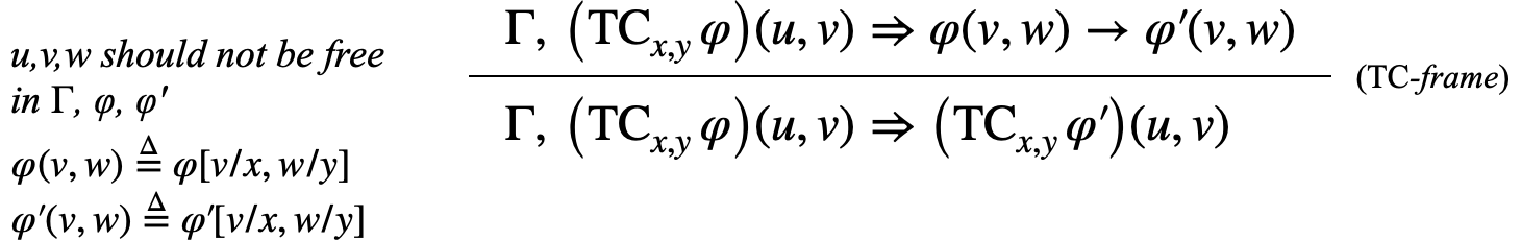
\includegraphics[width=10cm]{img/tc-frame-gen.pdf}
\caption{Generic frame property for (reflexive) TC}
\end{figure}

By developing proof-support tools that ``guess'' specific frame properties
% xref lemma speculation
and prove them automatically based on more primitive facts and by applying
generic frame properties, we expect to greatly improve the efficacy of theorem
provers and also of interactive proof assistants in handling conjectures
involving transitive closure.
While frame properties do not, formally, play any special role compared to
other formulas occurring throughout the proof, they follow a unique kind of
``thought pattern'' that serves a mental purpose in abstracting away nitpicky
details.
This would allow us to focus human and machine attention alike on the more
nitty-gritty parts of the proof.

\subsubsection{Next-level Transitive Closure}

The use of transitive closure logic is not restricted to reasoning about heap
graphs, which mostly involved low-level kind of reasoning.
Many aspects of computing rely on iteration, \eg when expressing properties of
aggregate data --- a sum of a column in a database, for instance.
Indeed, there is a large and interesting space of programs that can be realized
with the combination of the functional operations \textsf{map}, \textsf{filter},
and \textsf{reduce}. % cite SPARK
Sets and sequences can be stored in many ways in memory and in non-volatile
storage, yet the iteration aspect remains the same and can be characterized by
a ``next-in-iteration'' function that matches for each element, the following
element in the iteration order.
The loopy construct, \eg sum, can then be axiomatized using the transitive
closure $\big(TC_{\langle a,u\rangle,\langle b,v\rangle}v=n(u) \land b=a+\mathrm{val}(u)\big)$
With the help of TC support in the theorem prover, and in the presence of a
library of theorems defining known properties of TC, reasoning about such
aggregates can be streamlined to be simpler than by using the corresponding
inductive definition of sum.
For example, distributivity of sum over sequence concatenation follows (almost)
for free from the transitivity of TC.



\subsection{Modular Reasoning with Lemmas}

Mathematical proofs are seldom monolithic.
Usually, there are some intermediate conjectures --- \emph{lemmas} --- that
are proved one by one, gradually building toward the culmination of the main
theorem.
It is not done out of altruism towards potential readers of the paper, though it can
certainly make a proof easier to understand.
Mainly, it helps the author overcome the complexity of the proof development
task: in a formal setting, even a seemingly benign logical step can have many
inference steps; and the steps are not always sequential, for example when
a case split is required in order to consider several scenarios.

This kind of modularization has been carried over by computer scientists to the
realm of interactive proof assistants.
In Type Theory, the use of lemmas is wired in as they are reduced to function
calls following the Curry-Howard Correspondence.
Modular proofs are even more of the essence in automated proof search, due to
the inherent computational complexity of the tool and poor scalability of
existing search techniques.
Breaking a proof task into lemmas also carries the promise of combining different
approaches to finding the proofs, by applying a portfolio approach in the spirit
of Why3 \cite{}.

\subsubsection{...}

\subsubsection{Near-match Lemma Speculation}

The following is a common scenario for anyone who has worked on formal proof development:
you have a conjecture to prove, and there is
a theorem whose conclusion seems to fit the conjecture, but does not \emph{quite} match.
As a very simple example, suppose the conjecture is
$\exists k.~ n = 2\cdot k$, and the preexisting theorem states:
\begin{equation}\label{manna-divmod}
  \forall i, j.~ i = \fdiv(i, j) \cdot j + \frem(i, j)
\end{equation}

(Inspired by Manna and Waldinger, 1980.)
Strict syntactic unification would fail to apply (\ref{manna-divmod}) to the proof goal $n = 2\cdot \evar{k}$, since (\ref{manna-divmod}) has a $+$ operator on the right-hand side of the equality.
(Here and in the sequel, we use $\evar{k}$ to designate a pattern variable that can be unified with anything.)
However, an intelligent mathematician knows that according to the basic laws of arithmetic, $\forall x.~x + 0 = x$.
It is possible to ``unblock'' the unification process if we equate $\frem(\cdot,\cdot) = 0$.
Similarly, unifying $\fdiv(n,\evar{j})\cdot \evar{j}$ with $2\cdot \evar{k}$ would fail, since $2$ cannot be unified with $\fdiv(n,\evar{j})$.
Again, by the law of commutativity, 
$\fdiv(n,\evar{j})\cdot j = \evar{j} \cdot\fdiv(n,\evar{j})$,
so we should be able to unify $\evar{j}$ with $2$ and $\fdiv(n, 2)$ with $\evar{k}$.

This process of \emph{unification modulo equalities}, or \emph{E-unification}, has been explored in the past but never exploited for automation\citeneeded{}.

{\color{gray}
transitive closure (see above) of a unary function $n$.
Transitivity dictates that this follows from $n^*(x,v), n^*(v,z)$ for some $v$,
and there is an assumption, or a previously proven conjecture, $n^*(x,y)$;
however, no assumption $n^*(y,z)$ is available.
Instead, what you have is $m^*(y,z)$ for a second function $m$.
This can be overcome by proving that $m^*(y,z) \Rightarrow n^*(y,z)$, as a
separate lemma.
To prove such a lemma, one may try to prove that $n=m$, or that $n^*=m^*$,
or that $\forall u, n^*(y,u)\leftrightarrow m^*(y,u)$, or any other generalization
of the missing implication.}

To mechanize the process, a prover is required to select a suitable version.
Some alternatives can be vetted out using the model-based approach described
earlier.
Proving the auxiliary lemma can also be postponed to a later stage, after the
prover has concluded the current proof branch and admitted it --- since a failed
proof branch will be discarded anyway, and all the lemmas used in it become
moot.
Hence the term ``speculation'', also used in works on proofs by rippling \cite{}.
In the original presentation, speculated lemmas are equalities between terms,
but they can be made far more general and integrate
into any kind of clause-based inference system such as natural deduction or
sequent calculus used by modern provers.


\subsubsection{Semi-eager Theory Propagation}

The T of SMT stands for \emph{Theory}.
A theory in this context comprises of a specific vocabulary, inducing a limited
subset of logical formulas, and a designated interpretation, thus also limiting
the logical \emph{structures} that can be considered for them.
One popular example, built into many SMT solvers, is the theory of integer linear
arithmetic (LIA): it provides the operators ``$+$'', ``$-$'', ``$\cdot$'' as
well as order relations ``$=$'', ``$\leq$''.
It imposes a syntactic restriction that two variables may not be multiplied;
a variable may only be multiplied by a constant numeric literal.
While a formula such as $5 < 3$ is \emph{logically} satisfiable, it is
unsatisfiable in the theory of LIA, since it requires all numeric literals to
be interpreted as the integers they represent and that ``$<$'' be interpreted
as the order of integers.

Communication between the SAT component and the theory component of the model
is handled by the theory solver producing \emph{learned clauses} that are valid
modulo the theory and a logically unsatisfiable when conjoined with the existing
goal.
For $5 < 3$, this may be as simple as $\lnot(5 < 3)$; but the clauses get more
involved as problem sizes and number of variables grow.
The generation of clauses by the theory solver is called
\emph{theory propagation}, and can be done in two ways: (i) \emph{eagerly}, by
observing the formula given to the solver and generating all the theory-valid
statements containing the terms it contains; and (ii) \emph{lazily}, waiting for
SAT to produce a Boolean assignment and then contradicting it with
appropriate clauses when it is inconsistent with the theory.

The eager approach has an inherent flaw: the number of such theory-valid
statements can grow very large very quickly.
It can be infinite, in the case of some theories, as most theories are
represented, conceptually speaking, by quantified formulas, and there is no
bound on the number of instantiations that may be needed to refute a single
statement.
Some theories, in particular those of integers, are not even definable by any
finite set of first-order formulas, quantified or otherwise.
Such difficulties cause eager propagation techniques to be all but abandoned.

The lazy approach, despite its popularity, can have severe run-time
implications.
It means that a number of SAT assignments have to be observed, and a
potentially computation intensive procedure consulted, to refute their
satisfiability in the logic.
Designers of SMT try to be clever in the way propagation clauses are generated,
since generating more general clauses will drive the SAT away from more
inconsistent assignments at an earlier stage, saving calls to theory solver.
This tactic is limited, however, since the theory solver only gets a glimpse
of a narrow case each time it is involved, and cannot make global decisions
based on the structure of the entire input problem.

We propose a middle ground, and that middle ground involves a more holistic view of the proofs.
In a combined setting where SAT, theories, and formal proof objects work
together, intermediate proofs being explored provide ample subformulas to
fertilize propagation.
We will define an \emph{integration metric} for propagation clauses, that
quantitively expresses how tightly coupled a potential clause is with the
existing set of assumptions and goals present in the proof.
This can be thought of as a miniature ``page rank'' for logical formulas:
``hot'' atomic formulas, that is, ones that occur often in the proof, encourage
clauses that contain them, and these clauses, if accepted, will light up
more atomic formulas, with rank diminishing as they drift further from the
core.
Then, we will construct effective algorithms for finding such clauses that
optimize this metric.
We will tune the metric and the algorithms to achieve the fastest convergence
and compare to existing heuristics.

This semi-eager propagation of clauses from theories hold true potential for
a breakthrough with respect to handling theories and quantified conjectures
in unison, as challenged by Voronkov \citeneeded{}.


\subsubsection{Lemma Patching}

Again, this is inspired by the way mathematicians work, first proving a
simplified version of a desired property as a lemma, then inspecting the proof
to figure out ``what would go wrong'' in the more general case --- using that to guide insight toward
proving a stronger lemma.
Intermediate proofs are thus raw material for more proofs: this lends a
``white-box'' view of lemmas, complementing the more basic use of lemmas in
their closed form, encapsulating their proofs (which can be seen as
``black-box'').
In a dual manner, occasionally a lemma is too strong: \eg, if its conclusion is
a conjunction, but one is only interested in one of the conjuncts.
It is possible that a subset of the premises is sufficient to prove that one
conjunct.
Another example is when a conclusion is of the form $a < b$, but a relaxed set
of premises is enough to obtain $a \leq b$.

Moreover, during proof exploration itself (either by human or by machine), some
incorrect, dead-end proofs are inevitably encountered.
These are characterized, indeed identified, by assumptions that cannot be made
soundly (\eg a proof branch that includes formulas that are not logically valid).
Normally, a theorem prover simply discards these failed attempts and tries
other directions.
However, these too can be leveraged as raw material; repairing them amounts to
eliminating the spurious, invalid assumptions.

\begin{figure}
\centering
\raisebox{-.33\height}{
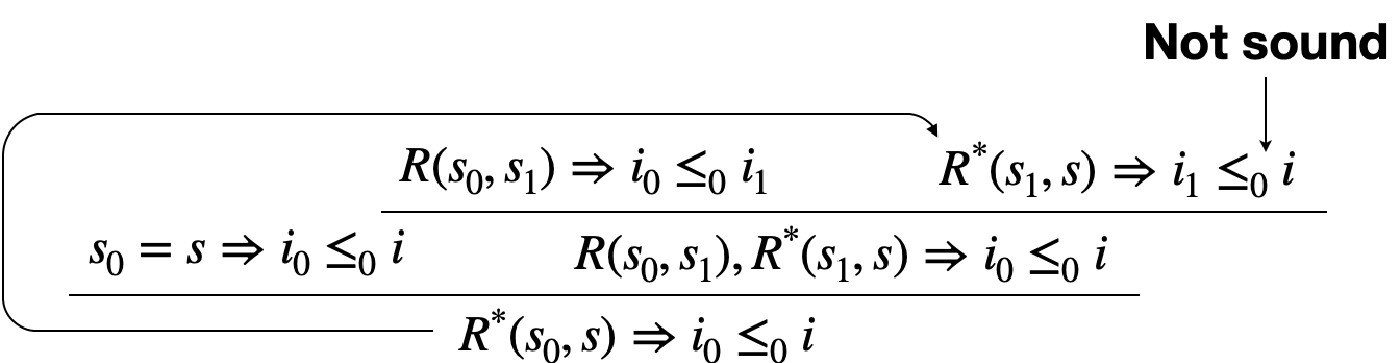
\includegraphics[width=7cm]{img/lemma-patching.pdf}}
$\longrightarrow$~~
\raisebox{-.33\height}{
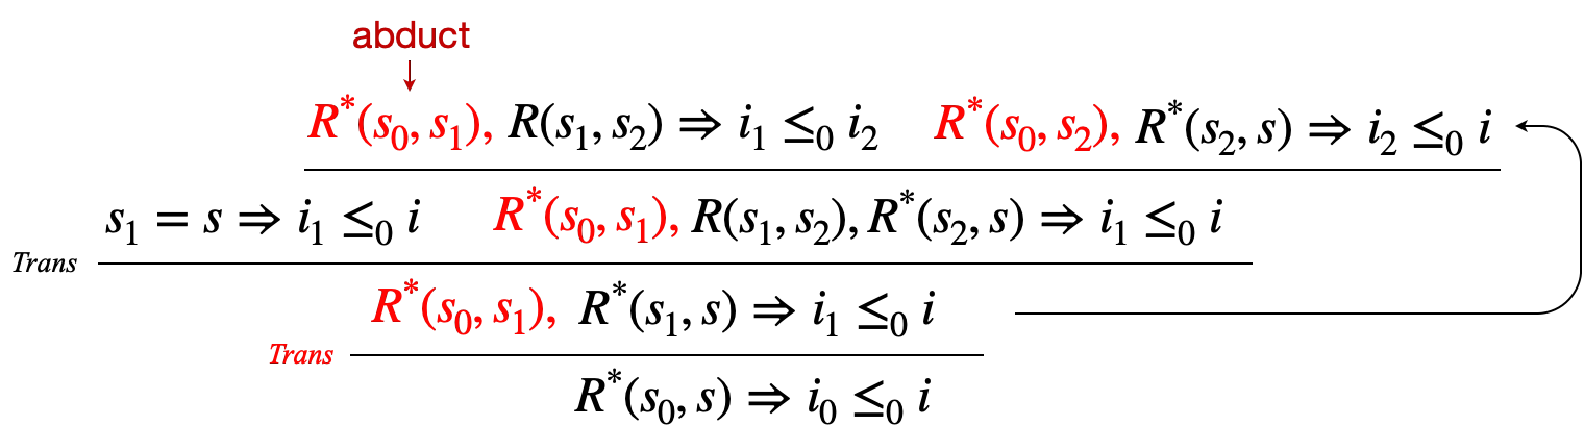
\includegraphics[width=7.5cm]{img/lemma-patching-abduct.pdf}
}
\caption{Example for lemma patching}
\label{lemma-patching-example}
\end{figure}

\todo{refer to \autoref{lemma-patching-example}}


\subsection{Extraploating to Software}

As much as mechanical theorem proving is useful for formalizing mathematics, it has much wider and more exciting uses when it comes to reasoning about computer programs and their semantics.
To date, the most popular text on interactive theorem proving in Coq is the Software Foundations series~\citeneeded{}, a collaborative community
effort to formalize programming language concepts
and verification problems.
The example proofs and exercises in the textbook make some use of proof automation facilities existing in Coq.
These are, however, far from what can be offerred by dedicated automated provers and solvers.
This research aspires to bring such automated tools to a new level, in which they will be able to cope with these fundamental tasks naturally and directly.
Most importantly, that they will be capable of handling such formal definitions as occur in~\citeneeded{(SF again)} naturally, without requiring the user to translate their claims into a restricted logical fragment.

\subsubsection{Homotopy for Programs}

Homotopy Type Theory~\citeneeded{} is an emerging field of study offering a fresh view on Martin-L\"of  Type Thoery, in which type judgements are given
first-class-citizen status.
Types can be declared isomorphic, allowing terms of one type to be interpreted as the other type.
In the field of mathematics, homotopy is quite valuable, since it enables the transfer of knowledge (definitions and theorems) across related fields.
We claim an insight, that homotopy is predominant in software as well.
As such, it can be leveraged to many automated reasoning tasks revolving around computer programs.
We point out two situation in which homotopy arises naturally in programming.

\begin{paragraph}{Alternative representations}
Oftentimes, the same data can be described in more than one way.
This can arise from a discrepency between libraries, or an abstraction gap between specification and implementation levels.
\end{paragraph}